%%\documentclass[hyperref={colorlinks=true},10pt]{beamer}
\documentclass[green,compress,10pt]{beamer}
\usepackage[latin1]{inputenc}
\usepackage{textcomp}
\usepackage{beamerthemesplit,graphics,color,graphicx,amsmath,amssymb,mathrsfs}
%\usepackage{appendixnumberbeamer}
\usepackage{xcolor,subfigure}
\usepackage{url}
\usepackage{multimedia}
\usepackage{rotating}
\usepackage{colortbl}
\usepackage{pifont}
\usepackage[absolute,overlay]{textpos}
\usepackage{path}
 \usepackage{amsmath}
%\usepackage{feynmp}
\usepackage{underscore}
\newcommand{\ttbar}{$t\bar{t}$}
\newcommand{\ttbargamma}{$t\bar{t}\gamma\,$}
\newcommand{\invfb}{fb$^{-1}$}
\newcommand{\mtop}{m$_{\rm{top}}$}
\newcommand{\etmiss}{E$_{\rm{T}}^{\rm{miss}}$}
\newcommand{\pT}{p$_{\text{T}}$}
\newcommand{\vr}{V_{\rm{R}}}
\newcommand{\vl}{V_{\rm{L}}}
\newcommand{\gr}{g_{\rm{R}}}
\newcommand{\gl}{g_{\rm{L}}}
\newcommand{\fr}{F_{\rm R}}
\newcommand{\fl}{F_{\rm L}}
\newcommand{\fz}{F_{\rm 0}}

\newcommand{\fR}{$F_{\rm R} \;$}
\newcommand{\fL}{$F_{\rm L} \;$}
\newcommand{\fZ}{$F_{\rm 0} \;$}
\newcommand{\nz}{N_{\rm 0} \;}
\newcommand{\nl}{N_{\rm L} \;}
\newcommand{\nr}{N_{\rm R} \;}
\newcommand{\Nz}{$N_{\rm 0} \;$}
\newcommand{\Nl}{$N_{\rm L} \;$}
\newcommand{\Nr}{$N_{\rm R} \;$}

\definecolor{brightgray}{rgb}{0.95,0.95,0.95}

\mode<presentation>
{
 \setbeamertemplate{background canvas}[vertical shading][bottom=white!10,top=white!10]
 \usetheme{Ilmenau}
 \usecolortheme{riceowl}
 \usefonttheme[onlysmall]{structurebold}

 
 \setbeamertemplate{footline}{                                                                                    
                                                  
   \begin{beamercolorbox}[wd=\paperwidth,ht=2.55ex,dp=1ex,dp=1ex]{date in head/foot}                                                          
                  
 \hspace{1ex} \scriptsize{\insertframenumber / \insertpresentationendpage \hspace{2.99cm}  -- Top quark mass @ 13TeV --  \hspace{2.01cm} Sebastian Schulte }     
% \hspace{1ex} \scriptsize{\insertframenumber / 3 \hspace{3.85cm}  -- Status report: reprocessing --  \hspace{2.61cm} Andrea Knue}

 \end{beamercolorbox}}

 %    \end{beamercolorbox}}%                                        
 
}


\setbeamercolor{button}{bg=magenta,fg=black}

\definecolor{hellgrau}{rgb}{0.95,0.95,0.95}
\newcommand{\Tipp}[1]{\textcolor{blue}{Tipp:} #1}
\newcommand{\heading}[1]{\textcolor{blue}{#1}}
\newcommand{\kommentar}[1]{}
\beamertemplatenavigationsymbolsempty
\setbeamercovered{dynamic}

\begin{document}
\title[]{\bfseries{Measurement of the Top Quark Mass in 
	the\\ $t\={t}\rightarrow$ lepton+jets channel \\form $\sqrt{s}=13$TeV ATLAS data}}
\vspace{2cm}

\author{{{\bf Sebastian~Schulte}, Andrea~Knue, StefanKluth, Richard Nisius}}
%\date{Fourth Annual LHCP Conference \\ -- Lund, 13th-18th June 2016 --}

\frame{
\begin{textblock}{14}(0.75, 1.75)
\titlepage
\end{textblock}
\vspace{-1.05cm}
\begin{textblock}{6}(12.5, 12.9)
\begin{figure}
\centering
\subfigure{\includegraphics[width=0.3in]{Logo/Tum.jpg}}
\end{figure}
\end{textblock}

\begin{textblock}{7}(4.5, 8.9)
	\begin{figure}
		\centering
		\subfigure{
\includegraphics[width=1.75in]{Logo/MPPGr.png}}
	\end{figure}
\end{textblock}

\begin{textblock}{6}(11.5, 12.9)
\begin{figure}
\centering
\subfigure{
\includegraphics[width=0.3in]{Logo/ATLAS.png}}
\end{figure}
\end{textblock}
}


\section{Introduction}


\frame{
\frametitle{\bfseries{Why measuring the top-quark mass?}}
\begin{textblock}{8}(1.5, 2.3)	
	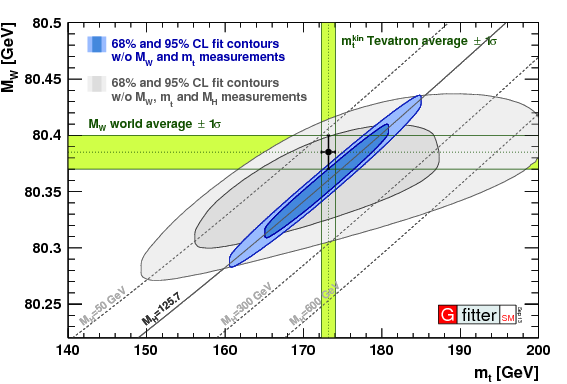
\includegraphics[width=0.9\linewidth]{PicsTop/EW}
	
	
\end{textblock}	

\begin{textblock}{6}(9.5, 2.3)	
		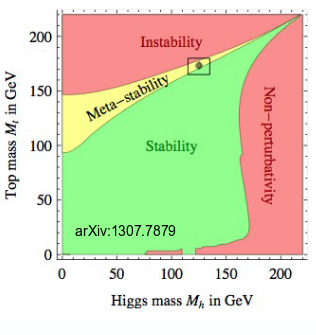
\includegraphics[width=0.9\linewidth]{PicsTop/Univ}
	

\end{textblock}	


\begin{textblock}{15}(2, 9.5)	
	
		\begin{itemize}
		\item Heaviest particle of the Standard Model (SM)
		\vspace{0.2cm}
			\item Top mass is close to electroweak symmetry breaking scale  
			\vspace{0.2cm}
			\item Significant contribution to radiative corrections
			\vspace{0.2cm}
			\item Important for physics beyond the SM
			\vspace{0.2cm}
			\item Important for the stability of our universe 
		\end{itemize}
	\end{textblock}	




\begin{textblock}{12}(7, 2.3)	

	
	
	
\end{textblock}	




}

\frame{
	\frametitle{\bfseries{Previous results}}
		\begin{textblock}{6.5}(0.5, 2.7)	
	
			\begin{alertblock}{World Comb. value (2014):}
				\begin{itemize}
					\item 	$m_{top} = 173.34 \pm 0.76$ GeV
				\end{itemize}
			
			\end{alertblock}
			
			\begin{alertblock}{l+jets measurements with 3D-template method:}
				\begin{itemize}
					\item 7 TeV (ATLAS): 	\href{https://twiki.cern.ch/twiki/bin/viewauth/AtlasProtected/TopMassNtuplesRun2}{\beamergotobutton{Top Mass Ntuple production}}	
					
				\end{itemize}
				
			\end{alertblock}
			
			
	\end{textblock}	

	
	
	\begin{textblock}{11}(6.5, 2.7)	
	
	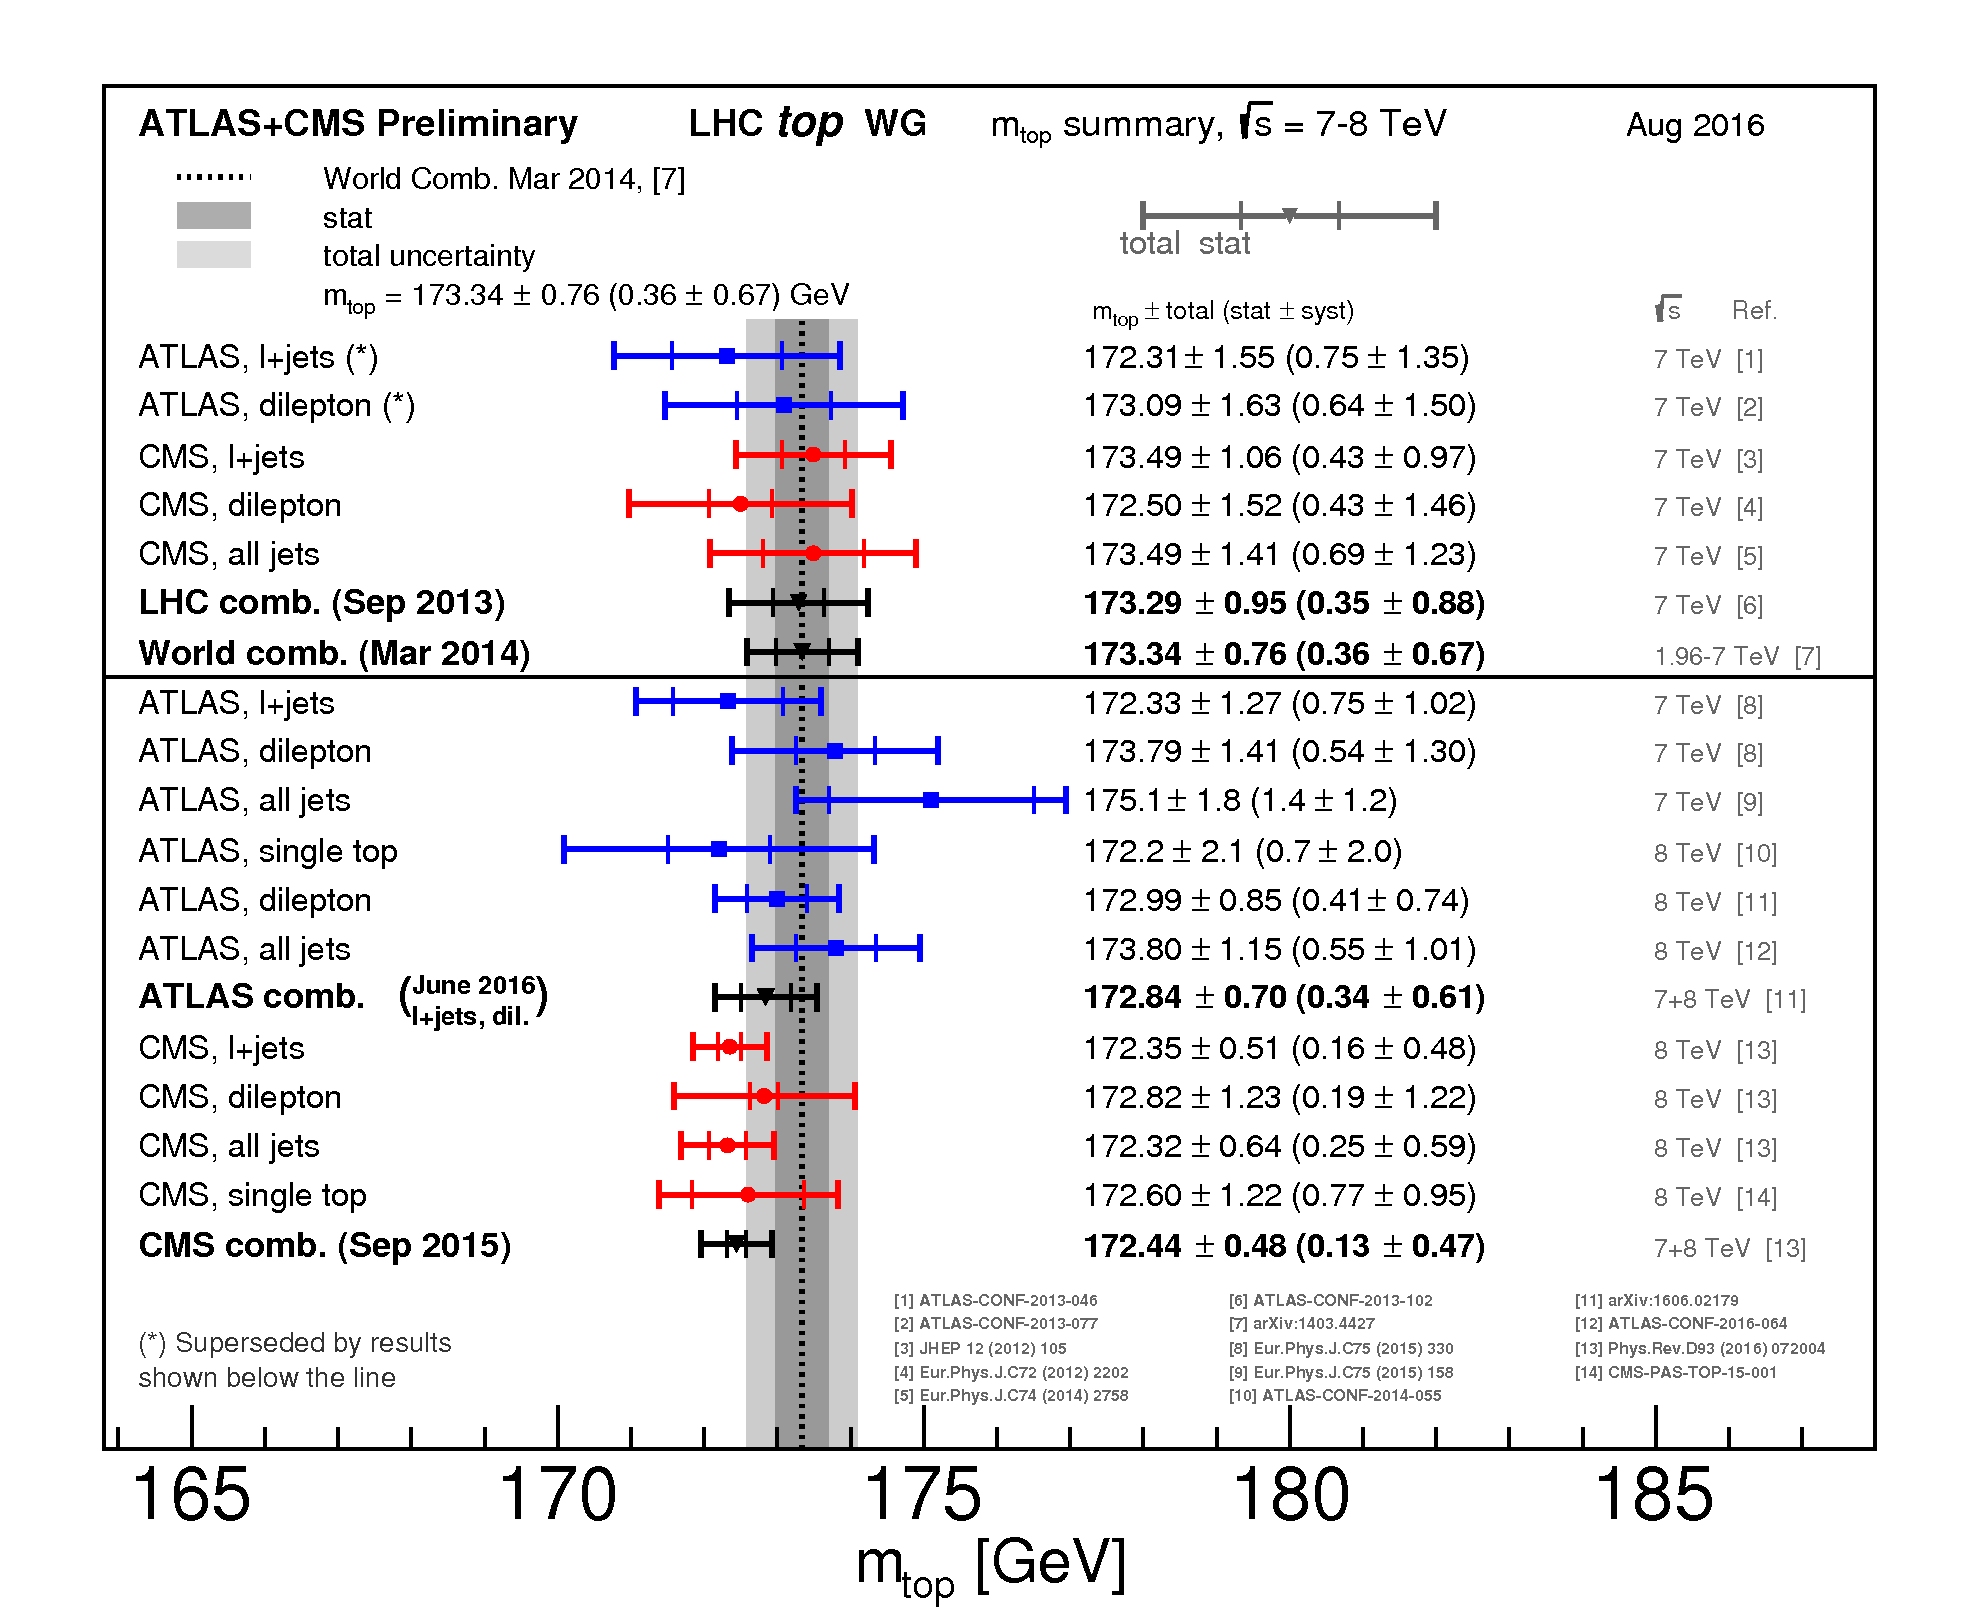
\includegraphics[width=0.8\linewidth]{PicsTop/mtopSum.png}
	
	
\end{textblock}	
}

\frame{
	\frametitle{\bfseries{How the Data is taken?}}
	
}
\frame{
	\frametitle{\bfseries{How is the top-qark mass measured?}}
	\begin{textblock}{18}(0.5, 2.8)	
	\bfseries{Measurement is based on a 3D-Template method:}
	\end{textblock}
\begin{textblock}{18}(0.5, 4.0)	
	\begin{itemize}
		\item Variable 1: $m_{top}^{reco}$ from reconstructed Events 
		\item Variable 2: $m_{W}^{reco}$ from chosen jet permutation, sensitive to JSF
		\item Variable 2: $R_{bq}^{reco}$ from chosen jet permutation, sensitive to bJSF
	
  \end{itemize}
	\end{textblock}
	
	
	\begin{textblock}{5}(2.5, 7.5)		
		
	
	
		$R_{bq} ^{reco,1b}= \frac{  p_{T}^{b_{tag}}    }{(p_{T}^{W_{jet1}} + p_{T}^{W_{jet2}})/2  } $
	
	\end{textblock}
	
		\begin{textblock}{5}(8.5, 7.5)		
			
			$R_{bq} ^{reco,2b}= \frac{  p_{T}^{b_{had}} + p_{T}^{b_{lep}}     }{p_{T}^{W_{jet1}} + p_{T}^{W_{jet2}}  } $
		\end{textblock}
		
	
	
	
	
	
	
	\begin{textblock}{9}(3.5, 9.5)	
		\begin{block}{Determination of $m_{top}:$}
			\begin{itemize}
				\item Need fully reconstruction of $t\={t}$-finale state
				\item Template parametrisation of the 3 variables
				\item Unbinned likelihood fit is performed
			\end{itemize}
		
		\end{block}
		\end{textblock}
	}
	

	
	

\frame{
	\frametitle{\bfseries{Workflow}}
	\begin{textblock}{18}(0, 2.5)	

		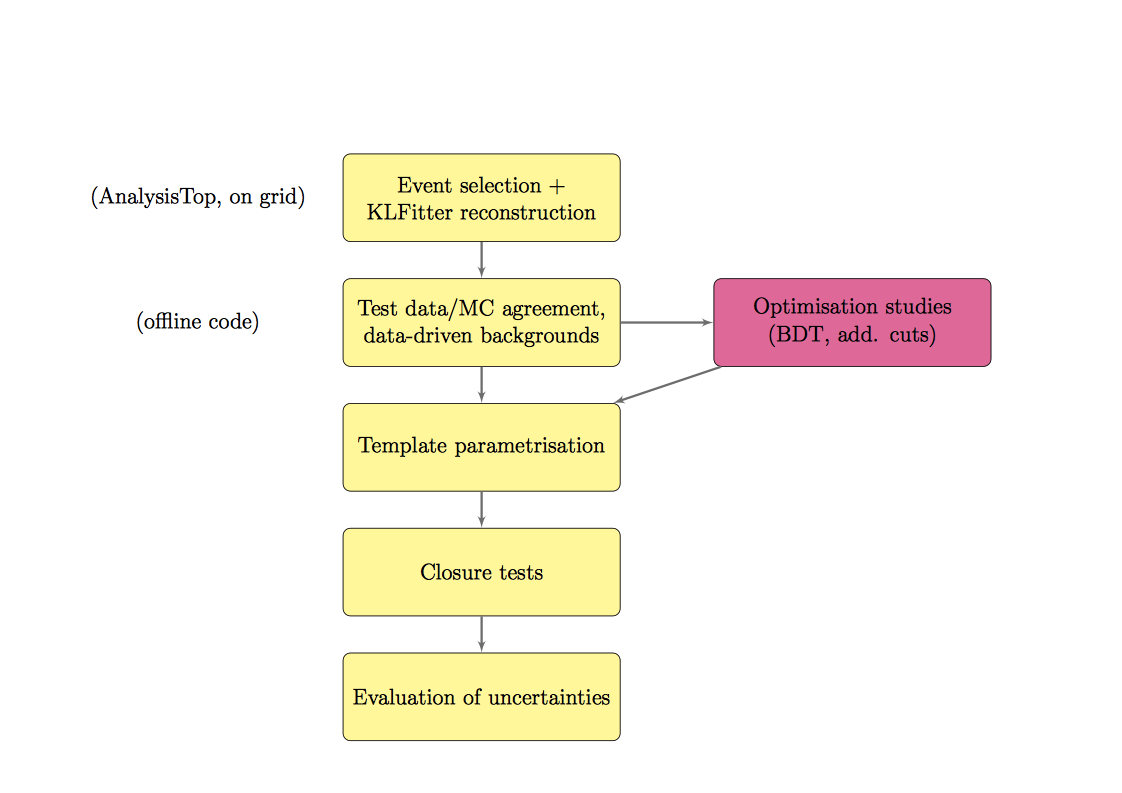
\includegraphics[width=0.7\linewidth]{PicsTop/Untitled 1.png}
		

	
	
		
	\end{textblock}	
	
}	




\frame{
	\frametitle{\bfseries{Pre-selection}}
	
	\begin{itemize}
		
		
		
		\item At least one good primary vertex with five associated tracks
		\vspace{0.2cm}
		\item Exactly one isolated high $ p_T$ lepton
		\vspace{0.2cm}
		\item At least 4 central jets with high$ p_T$ 
		\vspace{0.2cm}
		\item 1 or 2 b-tagged jets 
		\vspace{0.2cm}
		\item Cuts on   $E^{miss}_T$ ,  $m_T^W$  or  $E^{miss}_T$  + $m_T^W$             
		\vspace{0.2cm}
		\item W+jets normalization and HF fraction estimated from data
		\vspace{0.2cm}
		\item	Multijet background obtained from data in control region
		
		
	\end{itemize}
	
	
	
	
}


\section{Event selection}
%%%%%%%%%%%%%%%%%%%%%%%%%%%%%%%%%%%%%%%%%%%%%%%%%%%%%%%

%%%%%%%%%%%%%%%%%%%%%%%%%%%%%%%%%%%%%%%%%%%%%%%%%%%%%%%






\section{Data/MC agreement 13 TeV}

\frame{
	\frametitle{\bfseries{Event yields after pre-selection}}
	
	\begin{textblock}{19}(-1.25, 2.5)	
		\begin{center}
			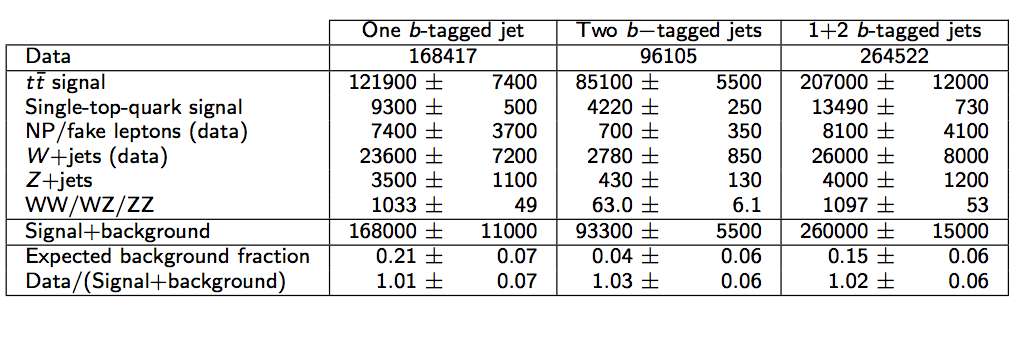
\includegraphics[width=0.8\linewidth]{PicsTop/Tab}
		\end{center}
		
\end{textblock}	
	
\begin{textblock}{18}(1.5, 9.5)	
	\begin{itemize}
		\item Background contamination dominated by W + Jets
		\vspace{0.2cm}
		\item Mass dependence of single-top $\Rightarrow $ include in signal
		\vspace{0.2cm}
		\item Reduction of background via cuts on 2 b-tagged jets
		\vspace{0.2}
		\item \bfseries{Good Data/MC agreement }
		 
	\end{itemize}
	
	
	
\end{textblock}
	
	
}


\frame{
	\frametitle{\bfseries{Data/MC agreement}}
	\begin{textblock}{5}(1.0,2.5)	
	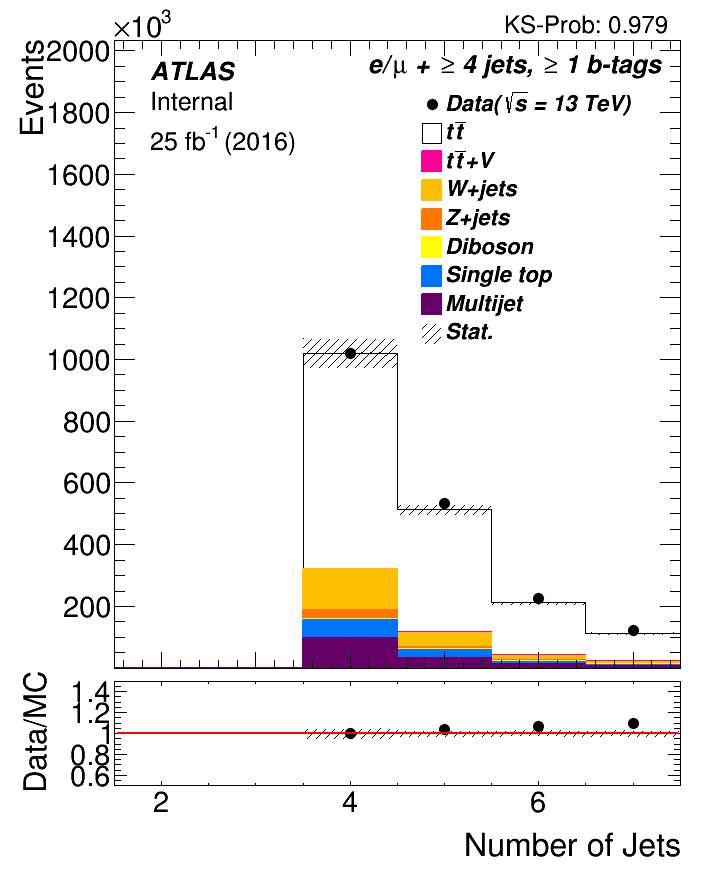
\includegraphics[width=0.8\linewidth]{PicsTop/1NumberJets.png}
	\end{textblock}

	\begin{textblock}{5}(6,2.5)	
	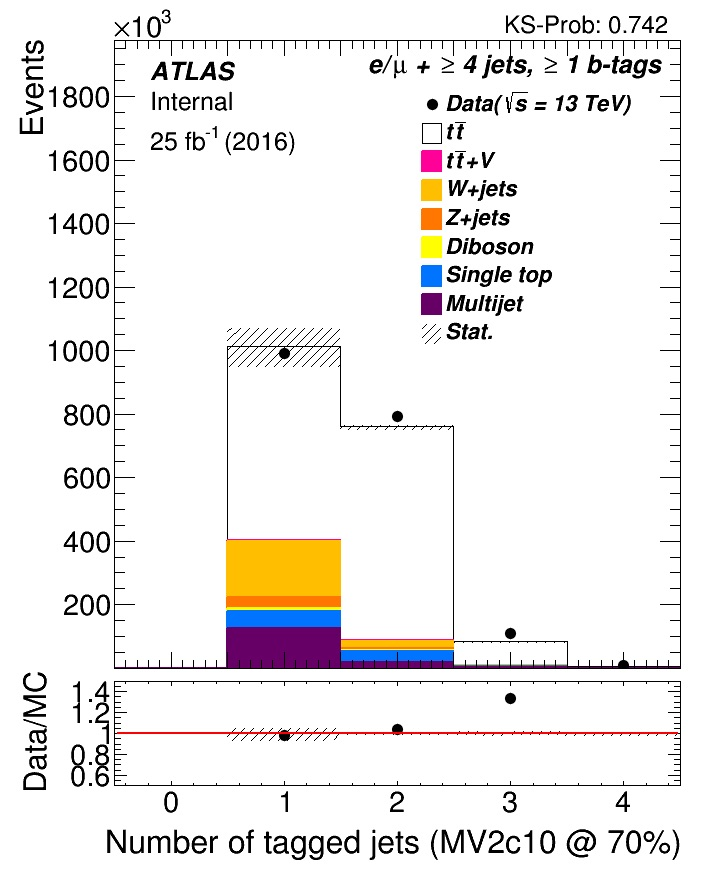
\includegraphics[width=0.8\linewidth]{PicsTop/1NJet.jpg}
	\end{textblock}

	\begin{textblock}{5}(11,2.5)	
	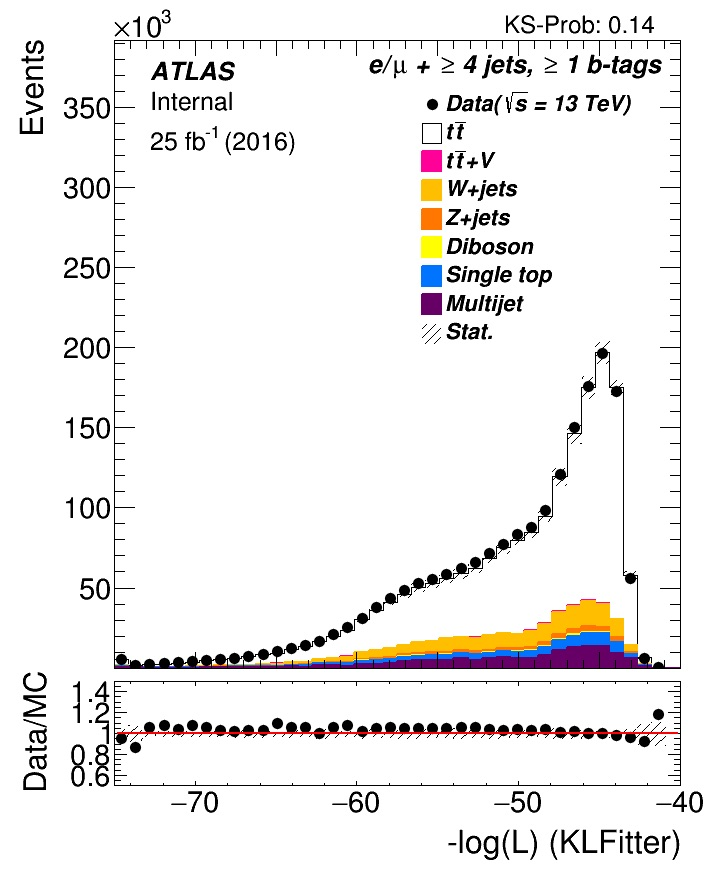
\includegraphics[width=0.8\linewidth]{PicsTop/logL.jpg}
    \end{textblock}
	
	\begin{textblock}{5}(1.0,9)	
	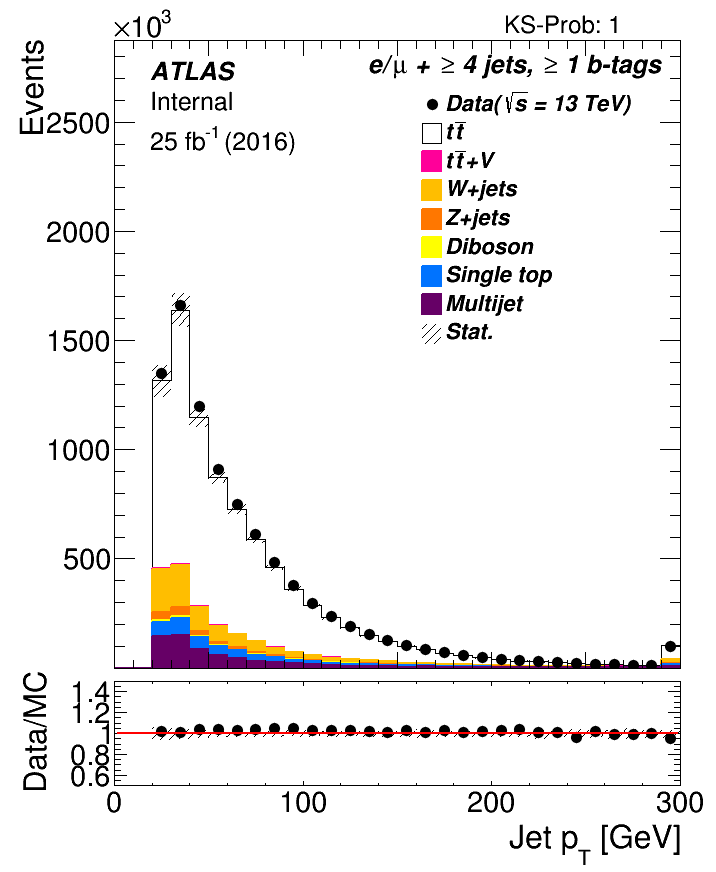
\includegraphics[width=0.8\linewidth]{PicsTop/jetpt.png}
	\end{textblock}
	
		\begin{textblock}{5}(6.0,9)	
		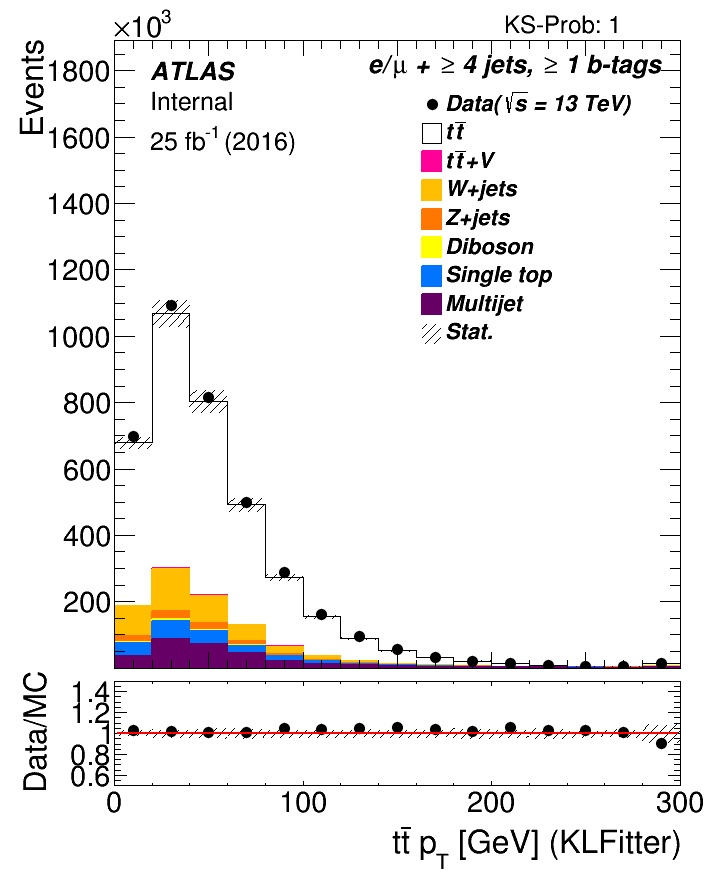
\includegraphics[width=0.8\linewidth]{PicsTop/ttbarpt.jpg}
	\end{textblock}

	\begin{textblock}{5}(11.0,9)	
	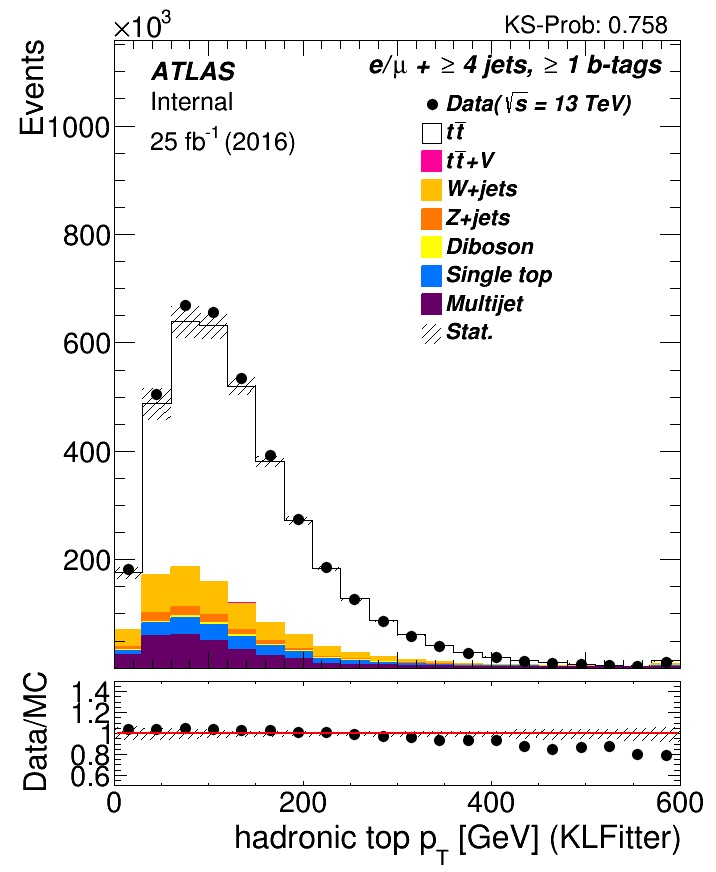
\includegraphics[width=0.8\linewidth]{PicsTop/hadpt.jpg}
\end{textblock}

}






	




\section{Event reconstruction}

\frame{
	\frametitle{\bfseries{$t\={t}$-final state}}

	\begin{textblock}{10}(2,2.5)
%	\begin{alertblock}
	\begin{itemize}
		
	
	\item 4 jet event $\Rightarrow$ 24 possible jet-parton assignments
	\vspace{0.2cm}
	\item 12 permutations left since light jets from W are  indistinguishable
	\vspace{0.2cm}
	\item Kinematic liklihood fit with KLFitter\\
	\vspace{0.2cm}
	$\Rightarrow$ \bfseries{choose best  permutations for calculation} 


	\end{itemize}
%\end{alertblock}
    \end{textblock}

	\begin{textblock}{10}(3.5,8)
		
			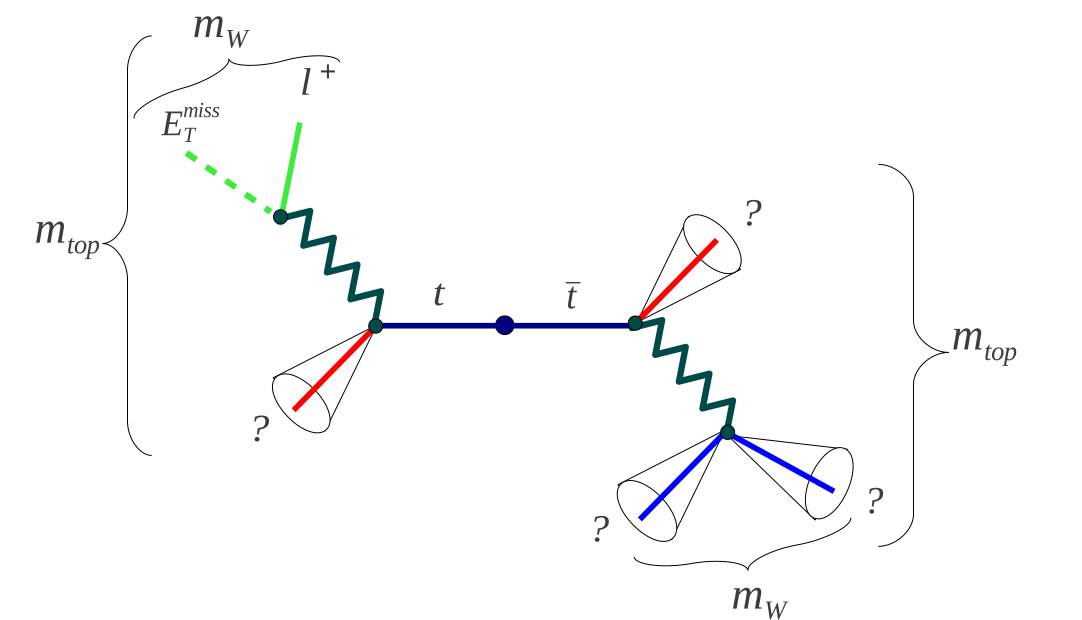
\includegraphics[width=0.9\linewidth]{PicsTop/Feynman.png}
	\end{textblock}	
 
}

\frame{
	\frametitle{\bfseries{Reconstruction with KLFitter}}
	\begin{textblock}{13}(0,2.5)
	\begin{itemize}
		\item KLFitter input: charged lepton, missing $E_T$ and at least four jets\\
		\vspace{0.2cm}
		
		$\Rightarrow$ one or two b-tagged jets + untagged jets with highest $p_T$
		\vspace{0.2cm}
		\item Definition of kinematic Likelihood:\\
		\begin{itemize}
			\item $W$: transfer functions for detector response
			\item $BW$:Breit-Wigner distributions 
			\item different options to use b-tagging information 
		\end{itemize}
			
	\end{itemize}
\end{textblock}
	\begin{textblock}{10}(3,8.5)
		\begin{block}{\bfseries{Likelihoodfunction}}
			
				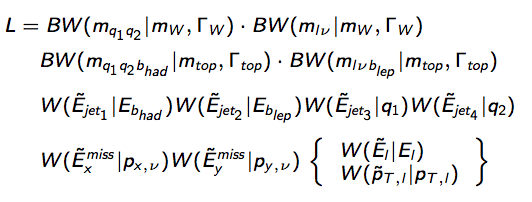
\includegraphics[width=0.9\linewidth]{PicsTop/Likeli}
			
			% $L = BW(m_{q_{1}q_{2}}|m_W, \Gamma _W)\cdot BW(m_{l\nu}|m_W, \Gamma _W)\cdot
			 %BW(m_{q_{1}q_{2}b_{had}}|m_{top}, \Gamma _{top})\cdot
			 %BW(m_{l\nub_{lep}}|m_{top}_, \Gamma _{top})\cdot
			% W(\~{E}_{jet_1}|E_b_{had})\cdot 
			% W(\~{E}_{jet_2}|E_b_{lep}) \cdot
			% W(\~{E}_{jet_3}|q_1) \cdot
			 %W(\~{E}_{jet_4}|q_2) \cdot
			 %W(\~{E}_{X}^{miss}|p_{X,\nu})\cdot
			 %W(\~{E}_{Y}^{miss}|p_{Y,\nu}) \begin{cases} W(\~{E}_{l}|E_l)  \\ W(\~{p}_{T,l}|p_{T,l})  \end{cases}
			
			
	
	\end{block}
	\end{textblock}
}

\section{Template parametrization} 
\frame{
	\frametitle{\bfseries{3D-template technique}}
		\begin{textblock}{15}(0.5,3)
	
		\begin{itemize}
			
			\item Simultaneous determination of $m_{top}, JSF$ and $bJSF$\\
			\vspace{0.2cm}
			$\Rightarrow JES/bJES$  uncertainties, become an additional statical component
			\vspace {0.2cm}
			\item Templates are derived for $m_{top}^{reco}, m_{top}^{reco}$ from MC samples
				\vspace {0.2cm}
			\item Construct templates as function of $m_{top}, JSF$ and $bJSF$ for signal and background
			
		
		
		\end{itemize}
	\end{textblock}



		\begin{textblock}{7}(0.5,8.5)
	\begin{block}{\bfseries{Fit (signal)}}
		\begin{itemize}
			\item $m_{top}^{reco}$:   gauss+ landau + landau$^{-1}$
		\vspace{0.2cm}
		\item $m_{W}^{reco}$: gauss + gauss
		\vspace {0.2cm}
		\item  $R_{bq}^{reco}$: gauss + gauss + landau
		
			
			
		\end{itemize}
		
		
	\end{block}
\end{textblock}




		\begin{textblock}{7}(8.5,8.5)
	\begin{block}{\bfseries{Settings}}
		\begin{itemize}
			\item $m_{top} \in \{ 170, 171.5, 173.5, 175 \}$ GeV
			\vspace{0.2cm}
			\item $JSF = 0.96-1.04$
			\vspace {0.2cm}
			\item  $JSF = 0.96-1.04$
			
			
		
	 	\end{itemize}
		
		
	\end{block}
\end{textblock}




}





\frame{
	\frametitle{\bfseries{Signal  $t\={t}$ only, 170 GeV $\&$ 171.5 GeV  }}
	\begin{textblock}{7.5}(0,2.25)
	
	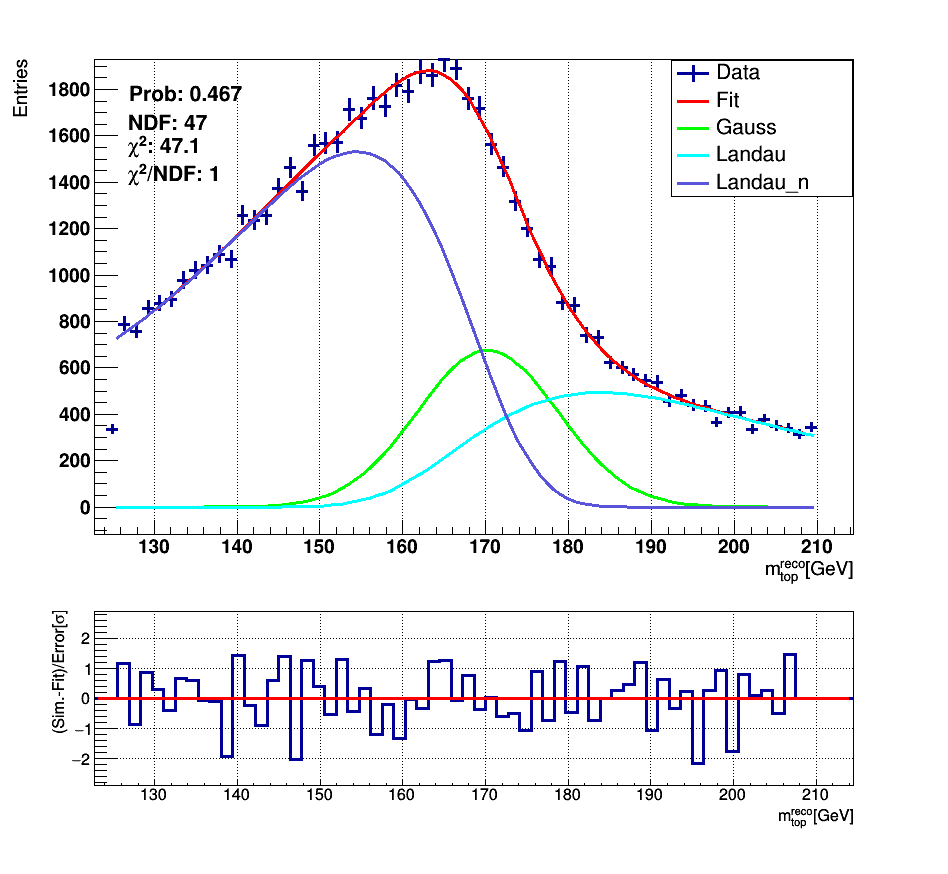
\includegraphics[width=0.725\linewidth]{PicsTop/170mtop.png}
	
	
	\end{textblock}	

	\begin{textblock}{7.5}(5.25,2.25)
	

		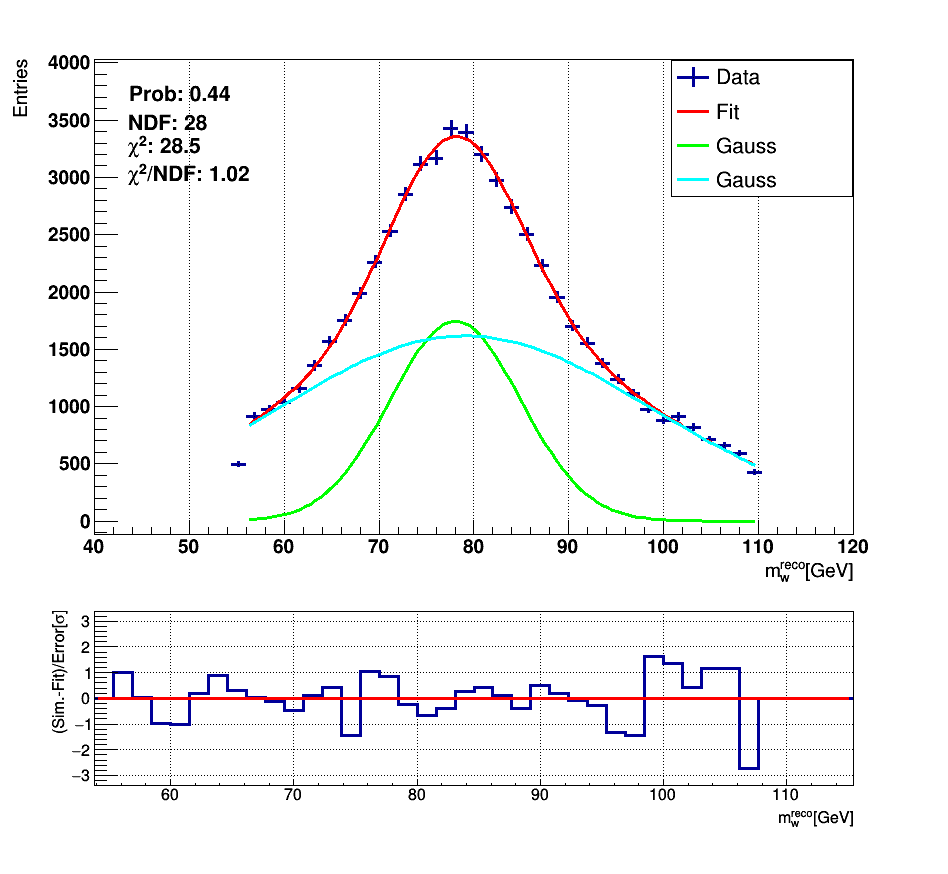
\includegraphics[width=0.725\linewidth]{PicsTop/170mw.png}
	
	
	
\end{textblock}	

	\begin{textblock}{7.5}(10.5,2.25)
	
	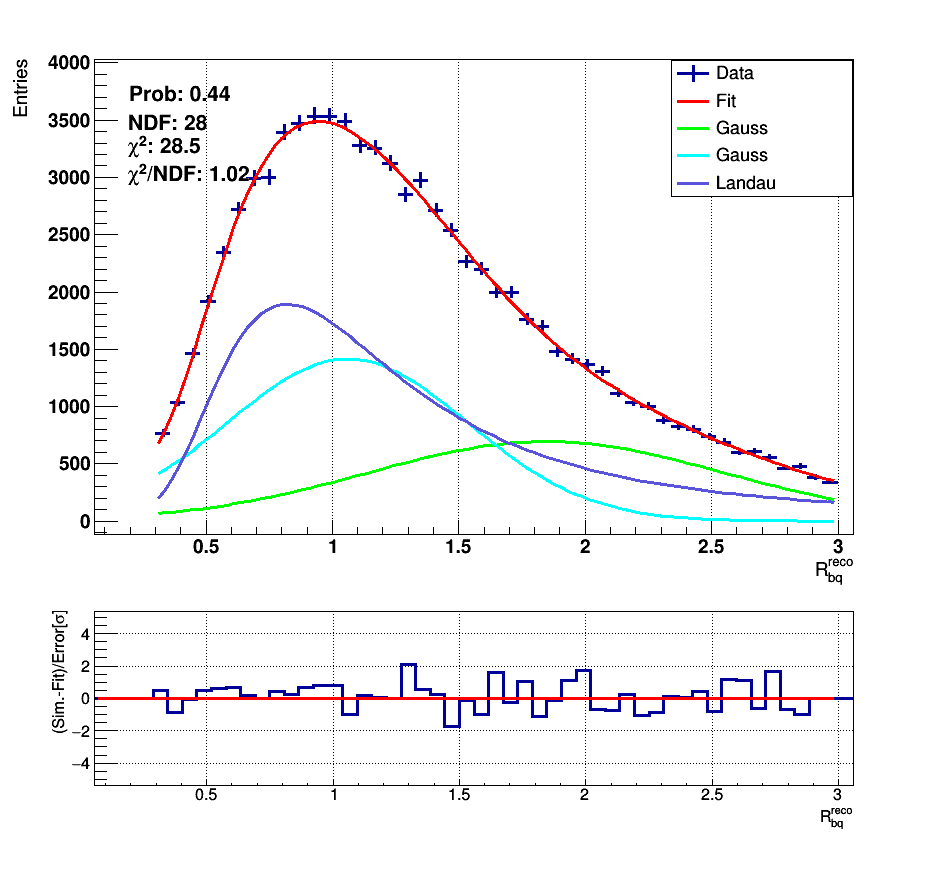
\includegraphics[width=0.725\linewidth]{PicsTop/170rbq.png}
	
	
\end{textblock}	




	\begin{textblock}{7.5}(0,8.75)
	
	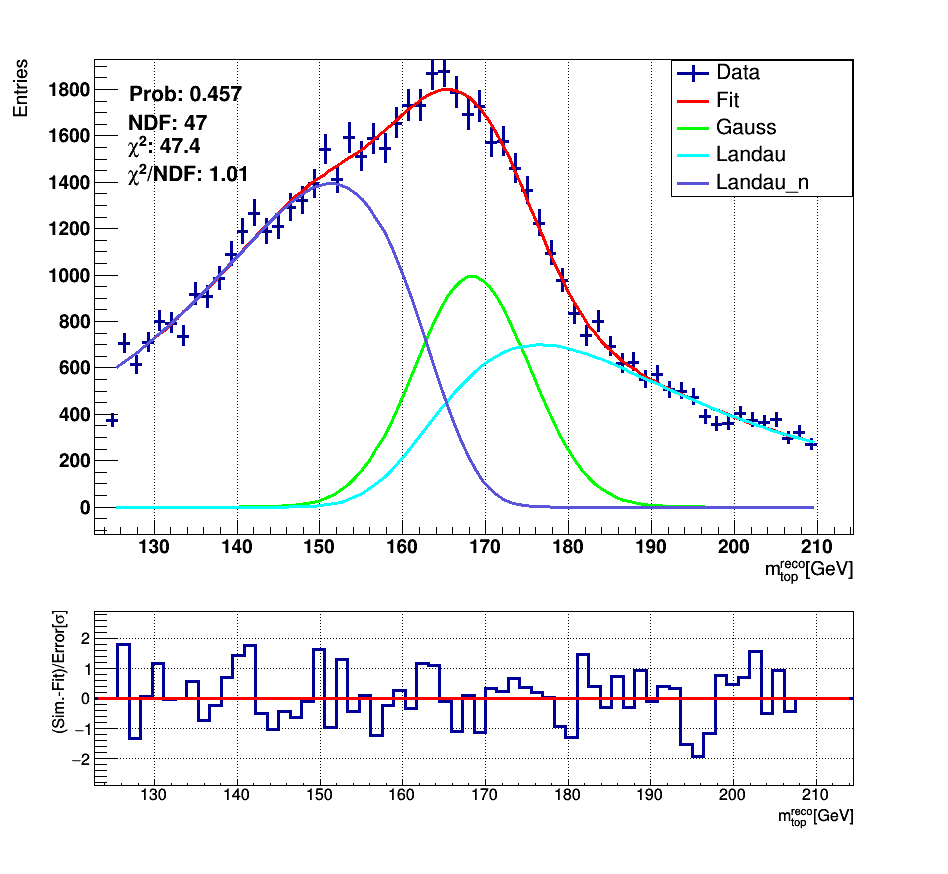
\includegraphics[width=0.725\linewidth]{PicsTop/171p5mtop.png}
	
	
\end{textblock}	

\begin{textblock}{7.5}(5.25,8.75)
	
	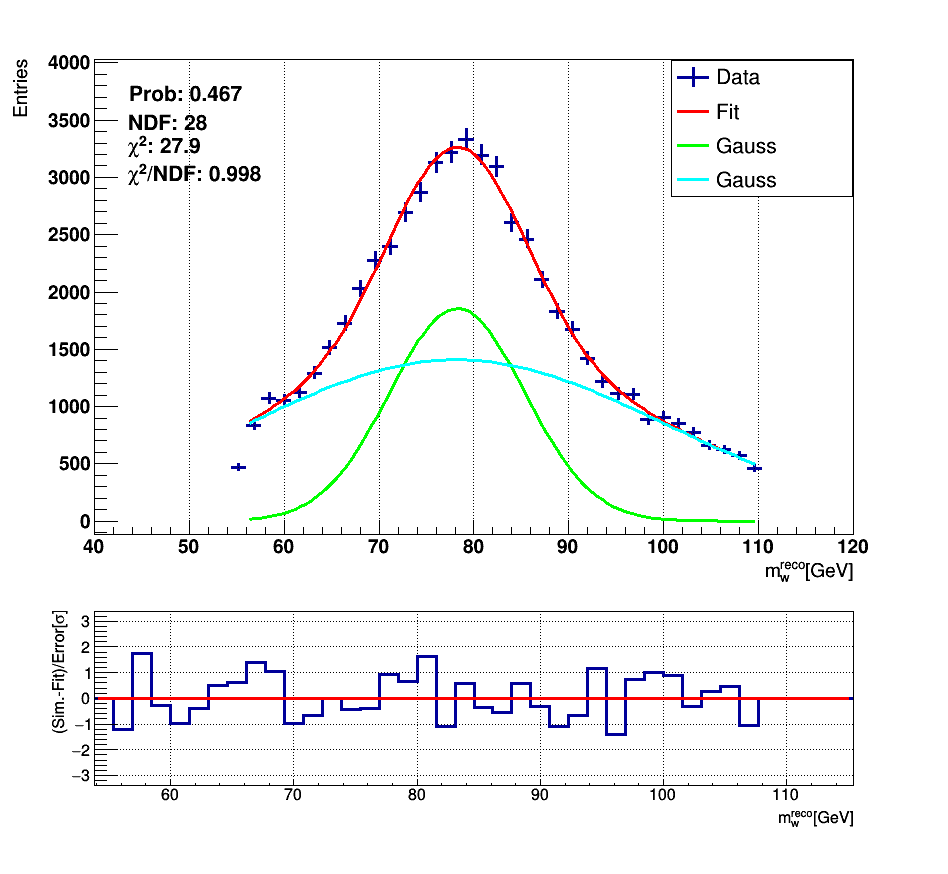
\includegraphics[width=0.725\linewidth]{PicsTop/171p5mw.png}
	
	
\end{textblock}	

\begin{textblock}{7.5}(10.5,8.75)
	
	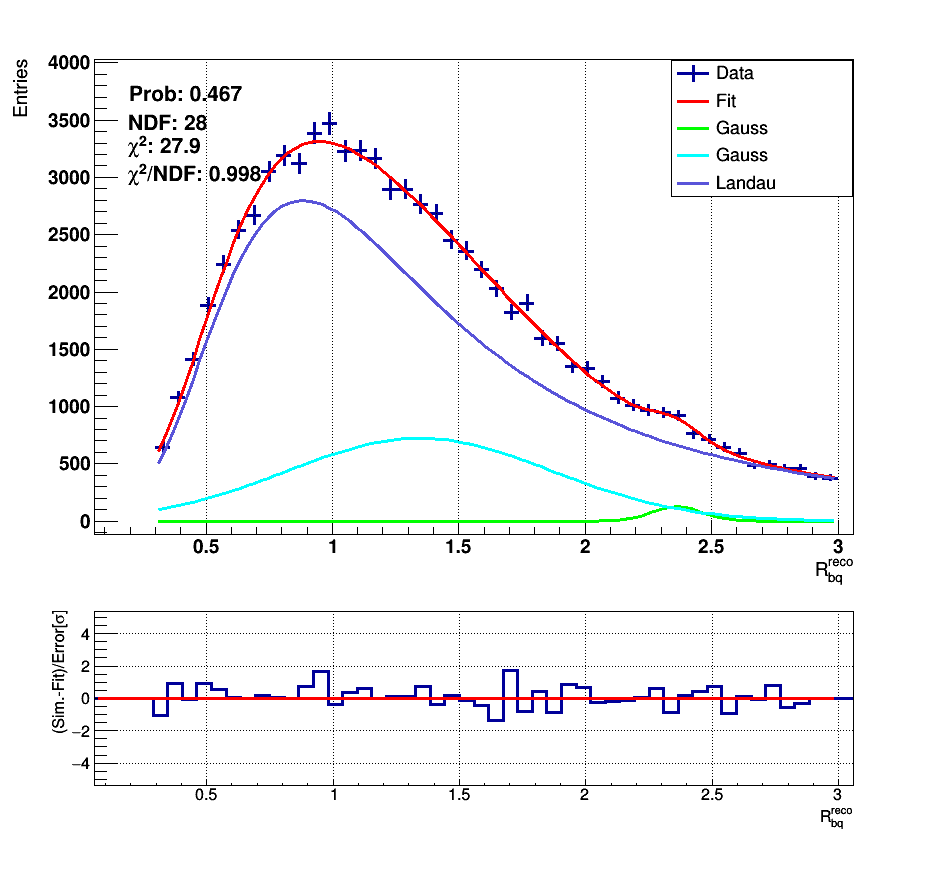
\includegraphics[width=0.725\linewidth]{PicsTop/171p5rbq.png}
	
	
\end{textblock}	

}

\frame{
	\frametitle{\bfseries{Signal  $t\={t}$ only,  173.5 GeV $\&$ 175 GeV }}
	\begin{textblock}{7.5}(0,2.25)
		
		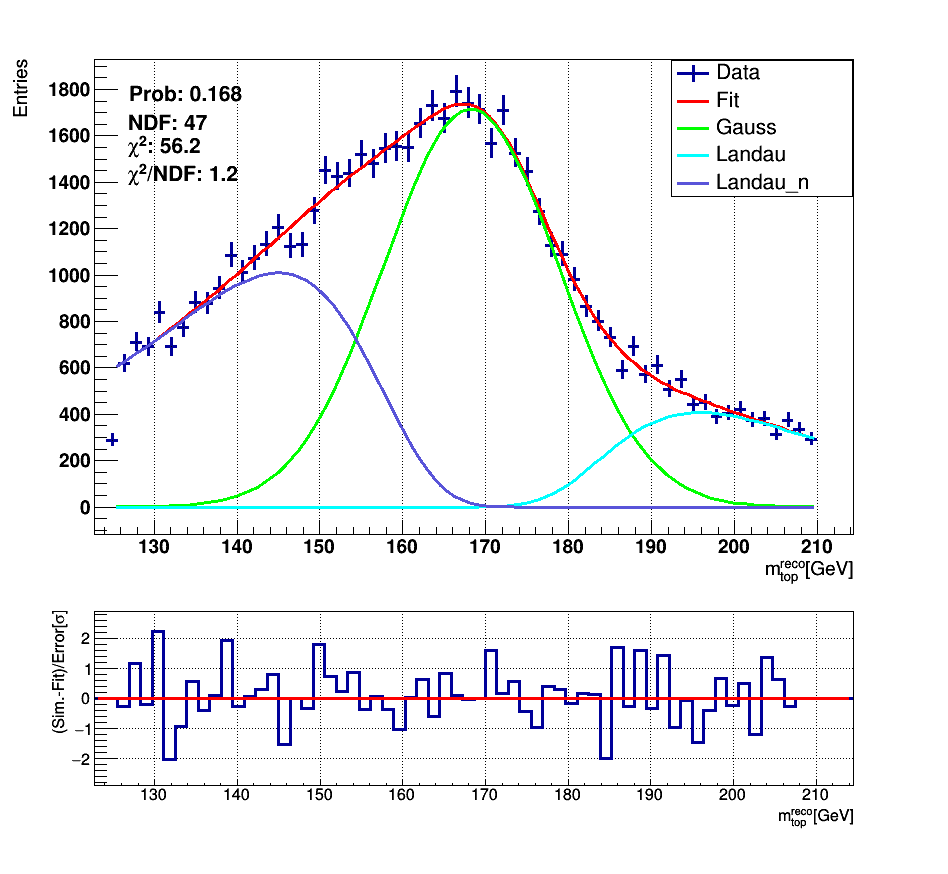
\includegraphics[width=0.725\linewidth]{PicsTop/173p5mtop.png}
		
		
	\end{textblock}	
	
	\begin{textblock}{7.5}(5.25,2.25)
		
		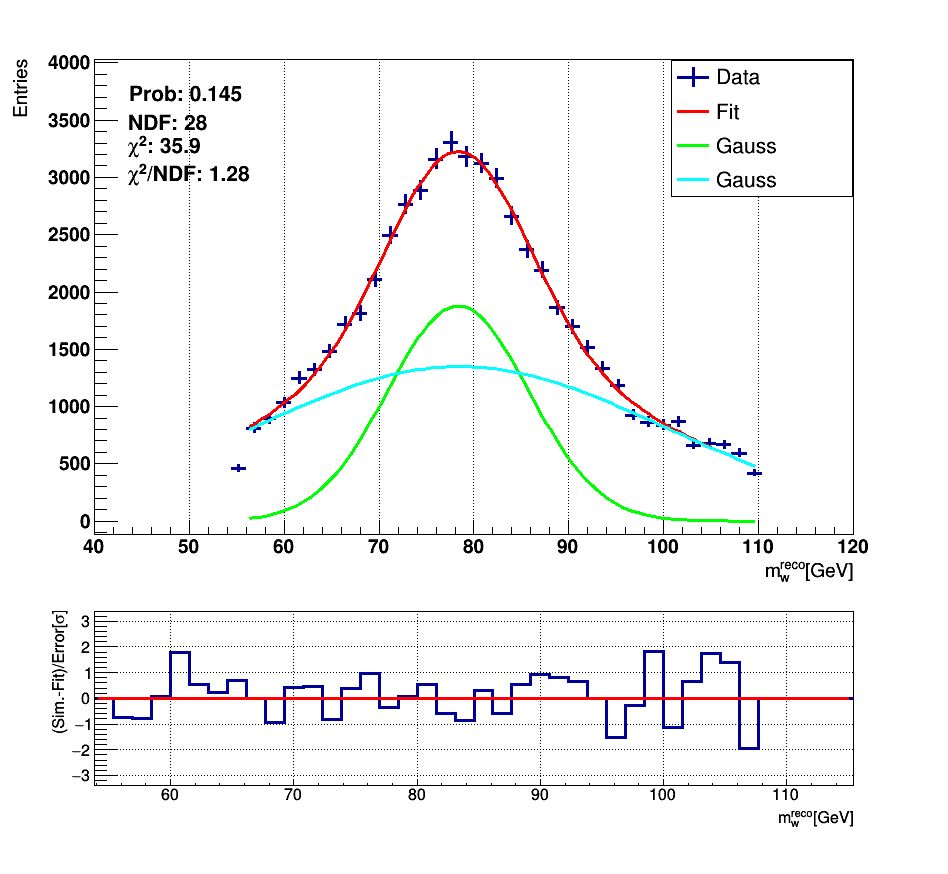
\includegraphics[width=0.725\linewidth]{PicsTop/173p5mw.png}
		
		
	\end{textblock}	
	
	\begin{textblock}{7.5}(10.5,2.25)
		
		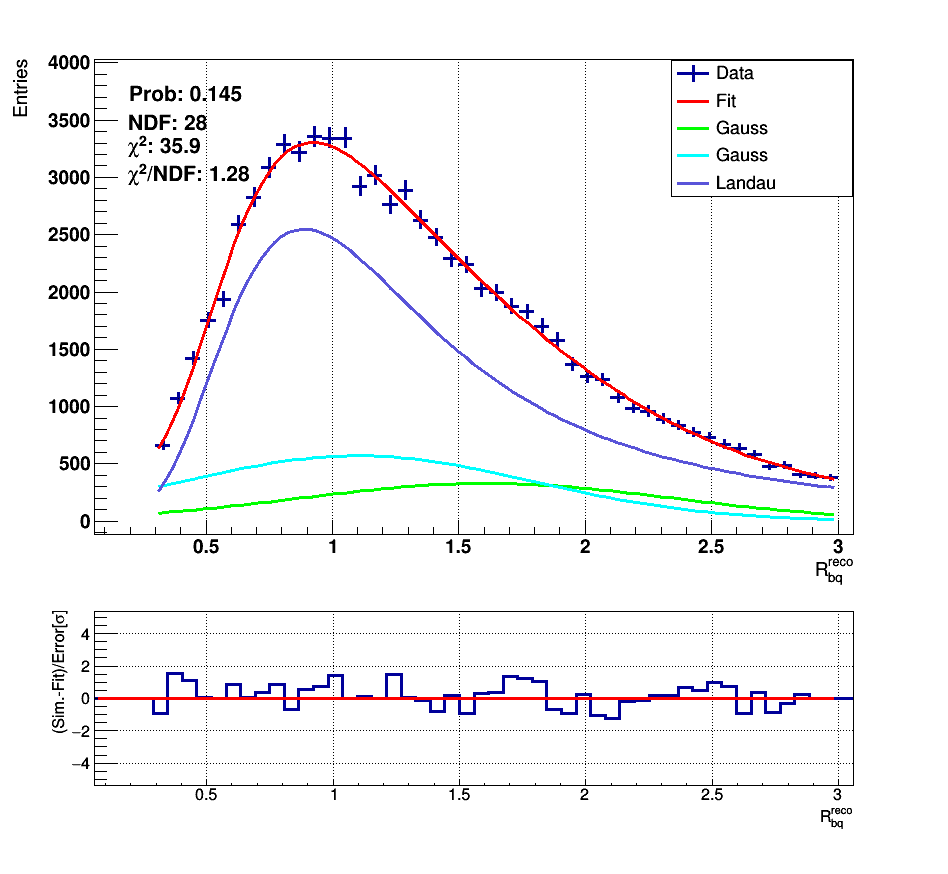
\includegraphics[width=0.725\linewidth]{PicsTop/173p5rbq.png}
		
		
	\end{textblock}	
	
	
	
	
	\begin{textblock}{7.5}(0,8.75)
		
		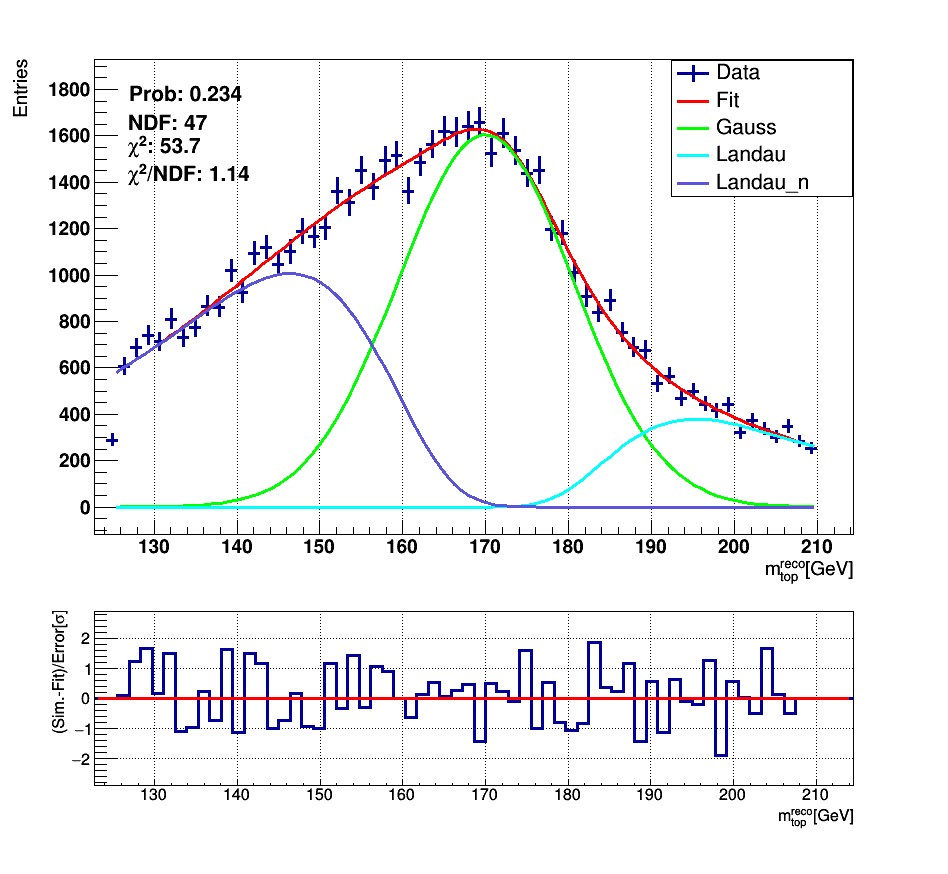
\includegraphics[width=0.725\linewidth]{PicsTop/175mtop.png}
		
		
	\end{textblock}	
	
	\begin{textblock}{7.5}(5.25,8.75)
		
		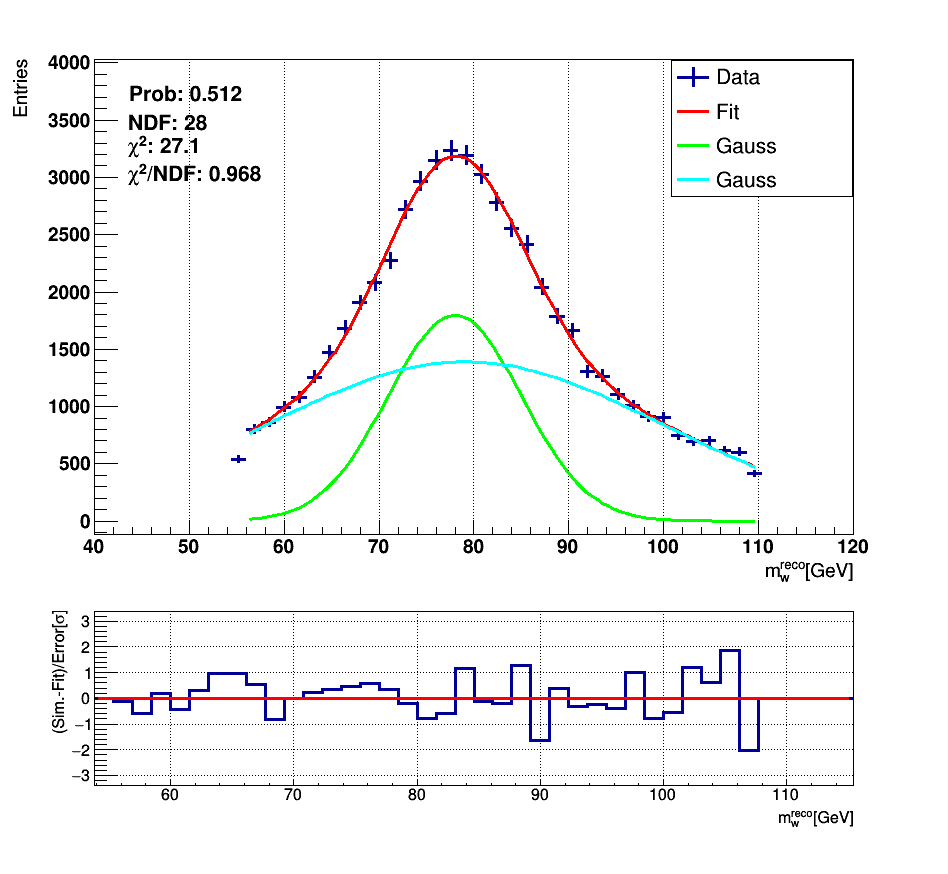
\includegraphics[width=0.725\linewidth]{PicsTop/175mw.png}
		
		
	\end{textblock}	
	
	\begin{textblock}{7.5}(10.5,8.75)
		
		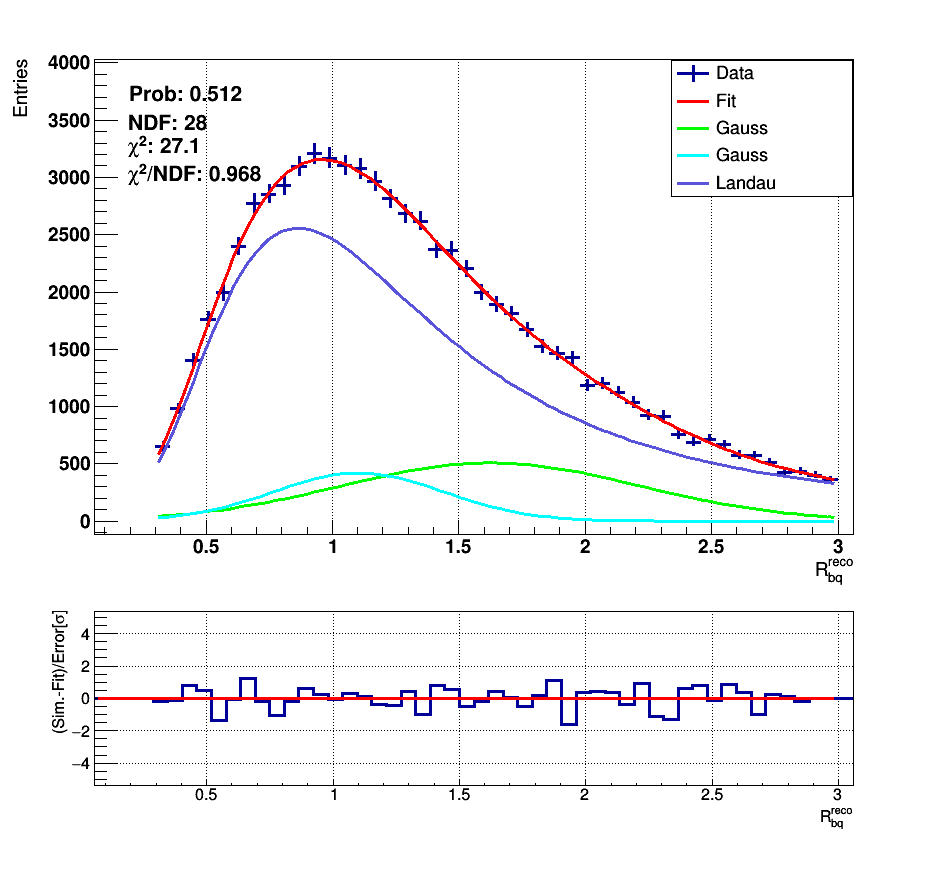
\includegraphics[width=0.725\linewidth]{PicsTop/175rbq.png}
		
		
	\end{textblock}	

}



\frame{
	\frametitle{\bfseries{Parameter interpolation $\&$ Likelihoodfit }}
	
		\begin{textblock}{15.5}(0.5,2.75)
		\begin{itemize}
			\item Single top contains additional information $\Rightarrow$ add to signal 
			\vspace {0.2cm}
		
			
			\vspace {0.2cm}

			\end{itemize}
			
		
			

		\end{textblock}	
		\begin{textblock}{17.5}(1.5,3.75)
				\begin{alertblock}{
				$\Rightarrow$ \bfseries{dependences of $m_{top}^{reco}, m_{top}^{reco}$ and $R_{bq}^{reco}$  on $mtop, JSF \/bJSF$ }}
			\end{alertblock}
			
		\end{textblock}
	
\begin{textblock}{14.5}(0.5,5.75)	
	\begin{itemize}
		\item Finally,  an unbinned likelihood  to the observed data distribution is performed to determine  the physics parameter

	\end{itemize}
	
\end{textblock}	

	\begin{textblock}{14.5}(2,8)	
			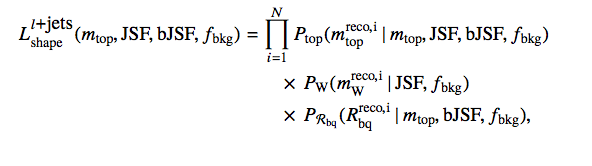
\includegraphics[width=0.725\linewidth]{PicsTop/Like}
		
	\end{textblock}	
	
	\begin{textblock}{14.5}(0.5,12.5)	
		\begin{itemize}
			
	
				\item Verification of the internal fitting consistency via pseudo-experiments
		
		\vspace {0.2cm}
		
		\item Optimization of the analysis to reject combinatorial background 
			\end{itemize}
\end{textblock}	
	
}



\frame{
	\frametitle{\bfseries{Summery $\&$ outlook}}
	\begin{textblock}{15}(0.5, 2.5)	
		\begin{alertblock}{Current status}
			\begin{itemize}
				\item Did several vent selection and reconstruction with 13 TeV samples \\
				\vspace{0.1cm}
				$\Rightarrow$ data MC agreement: good for four jets one tag inclusive, except for b-tagging multiplicity, worse agreement for four jets, two b-tagged inclusive 
				\vspace{0.2cm}
				\item Implemented the template parametrisation for several $t\={t}$ signal samples \\
					\vspace{0.1cm}
				$\Rightarrow$ good description by the chosen functions,  fit converge for all $m_{top}$
				\vspace{0.2cm}
				
				
			\end{itemize}
		\end{alertblock}
		\end{textblock}	

			\begin{textblock}{15}(0.5, 9.5)	
			\begin{alertblock}{Next steps}
				\begin{itemize}
					\item Include single top into the signal fits \\
				
				
					\vspace{0.2cm}
					\item Perform the fit for all $JSF$ and $bJSF$\\
					
					\vspace{0.2cm}
					\item Use probability density functions  for $m_{top}^{reco}$, $m_{W}^{reco}$  and $R_{bq}^{reco}$  in  unbinned likelihood fit to the data for all events
					
				
				\end{itemize}
			\end{alertblock}
		
		
	\end{textblock}	
	
}	






















\frame{
	\frametitle{\bfseries{Backup}}
	
	
	
}	

\frame{
	\frametitle{\bfseries{Object definition for 2016 data}}
	
	\begin{textblock}{7}(0.5, 2.5)	
		\begin{block}{\bfseries{Electrons}}
			\begin{itemize}
				\item $E_T > $28 GeV, $\mid \eta  \mid< $2.47
				\item Gradient isolation, TightLH
				\item HLT_e26_lhtight_nod0_ivarloos,
				HLT_e60_lhmedium_nod0, 
				HLT_e140_lhloose_nod0
			\end{itemize}
			
		\end{block}	
		
	\end{textblock}	
	
	\begin{textblock}{7}(0.5, 8.5)	
		\begin{block}{\bfseries{Small-R jets}}
			\begin{itemize}
				\item antiKt R = 0.4, EM-Jets
				\item JVT $>$0.59 for $p_T <$ 60GeV and $\mid \eta  \mid< $2.4
				\item b-tagging: MV2_c10, 77\% WP
			\end{itemize}
			
		\end{block}	
		
	\end{textblock}	
	
	
	
	
	\begin{textblock}{7}(8.5, 2.5)	
		\begin{block}{\bfseries{Muons}}
			\begin{itemize}
				\item $E_T > $28 GeV, $\eta < $2.47
				\item Medium, Gradient isolation
				\item HLT_mu26_ivarmedium,
				HLT_mu50
				\space
				\space
			\end{itemize}
			
		\end{block}	
		
		
	\end{textblock}	
	
	\begin{textblock}{7}(8.5, 8.5)	
		\begin{block}{\bfseries{MET/MTW}}
			\begin{itemize}
				\item $E_T^{miss} >$ 20GeV
				\item $E_T^{miss} + m_T^{W}>$ 60GeV
			\end{itemize}
			
		\end{block}	
		
	\end{textblock}	
	
	\begin{textblock}{17}(1.5,14.5)	
		\bfseries{AnalysisTop-02-04-27}, with 25 fb-1 for 2016 data
		\href{https://twiki.cern.ch/twiki/bin/viewauth/AtlasProtected/TopMassNtuplesRun2}{\beamergotobutton{Top Mass Ntuple production}}
	\end{textblock}
	
}

\frame{
	\frametitle{\bfseries{Signal templates $t\={t}$ only for 173.5 GeV $\&$ 175 GeV }}
	\begin{textblock}{7.5}(0,2.25)
		
		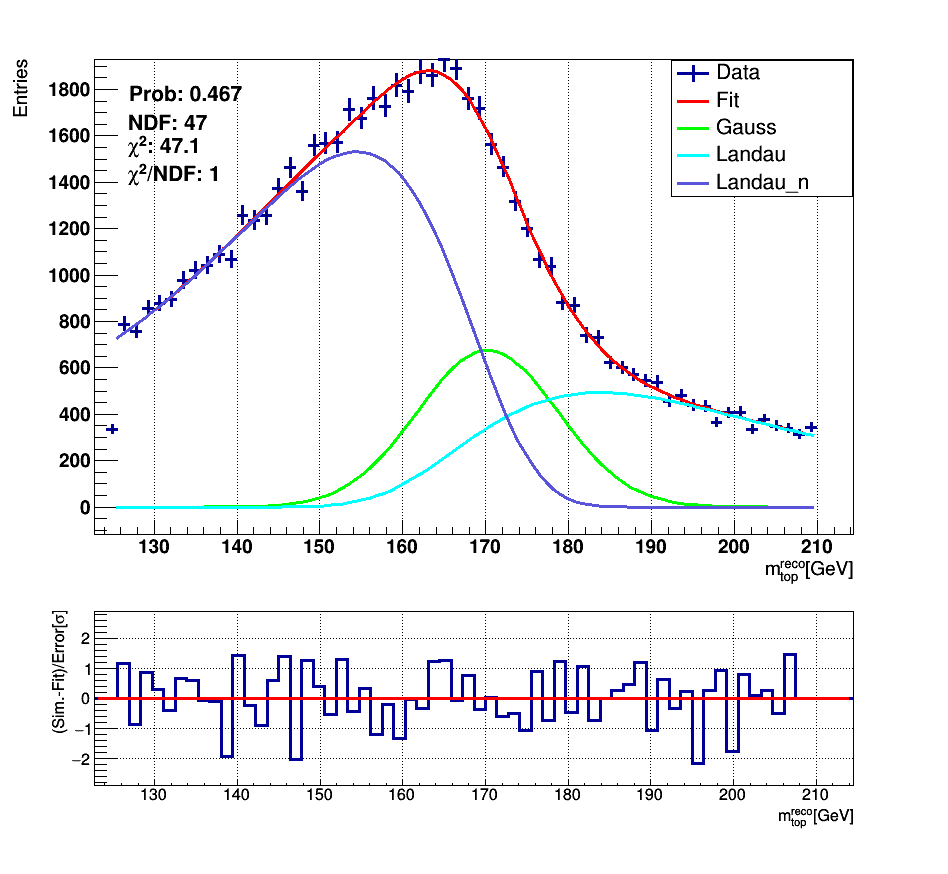
\includegraphics[width=0.725\linewidth]{PicsTop/170mtop.png}
		
		
	\end{textblock}	
	
	\begin{textblock}{7.5}(5.25,2.25)
		
		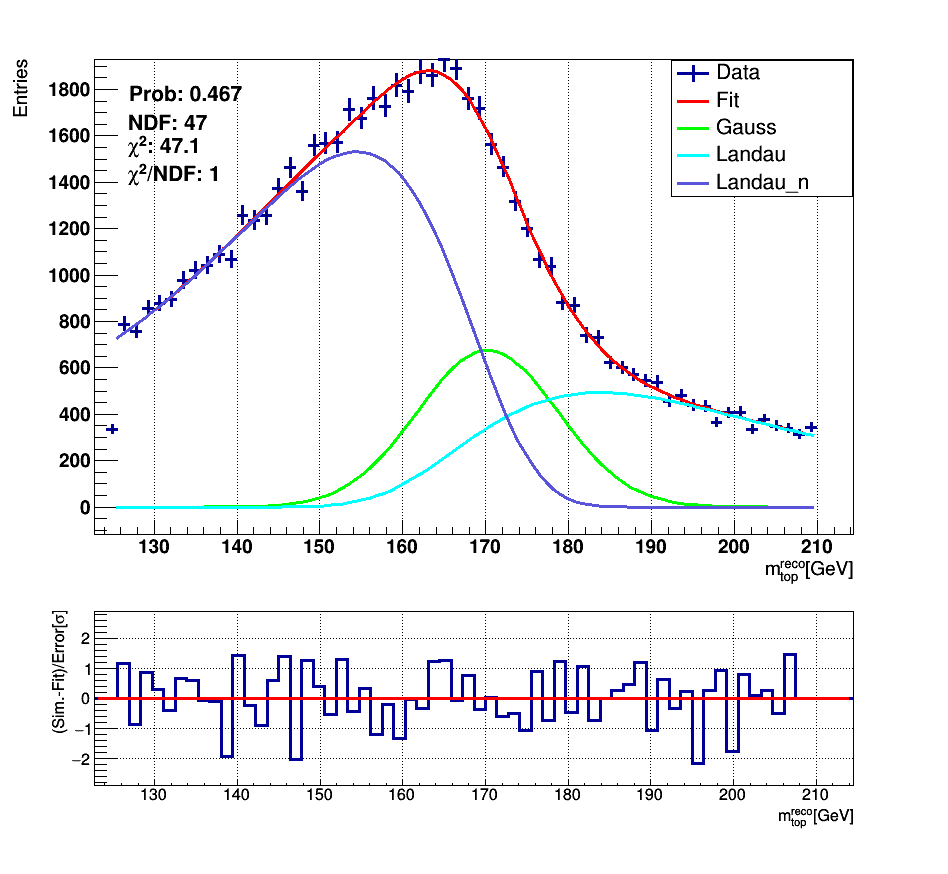
\includegraphics[width=0.725\linewidth]{PicsTop/170mtop.png}
		
		
	\end{textblock}	
	
	\begin{textblock}{7.5}(10.5,2.25)
		
		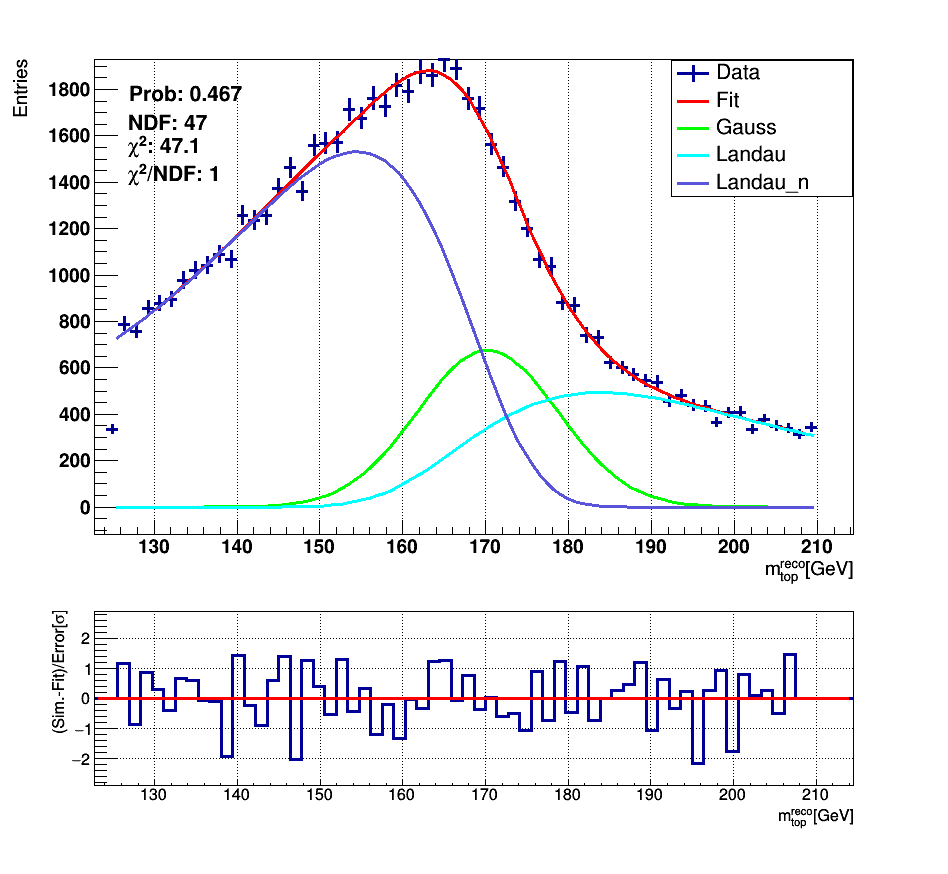
\includegraphics[width=0.725\linewidth]{PicsTop/170mtop.png}
		
		
	\end{textblock}	
	
	
	
	
	\begin{textblock}{7.5}(0,8.75)
		
		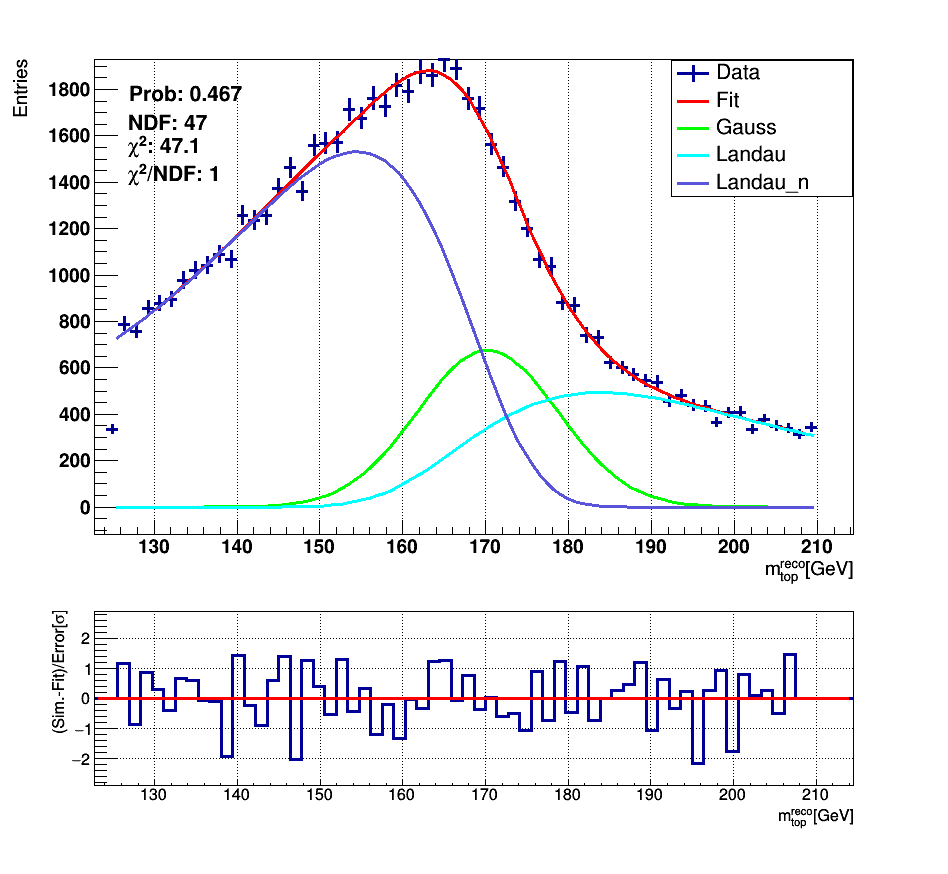
\includegraphics[width=0.725\linewidth]{PicsTop/170mtop.png}
		
		
	\end{textblock}	
	
	\begin{textblock}{7.5}(5.25,8.75)
		
		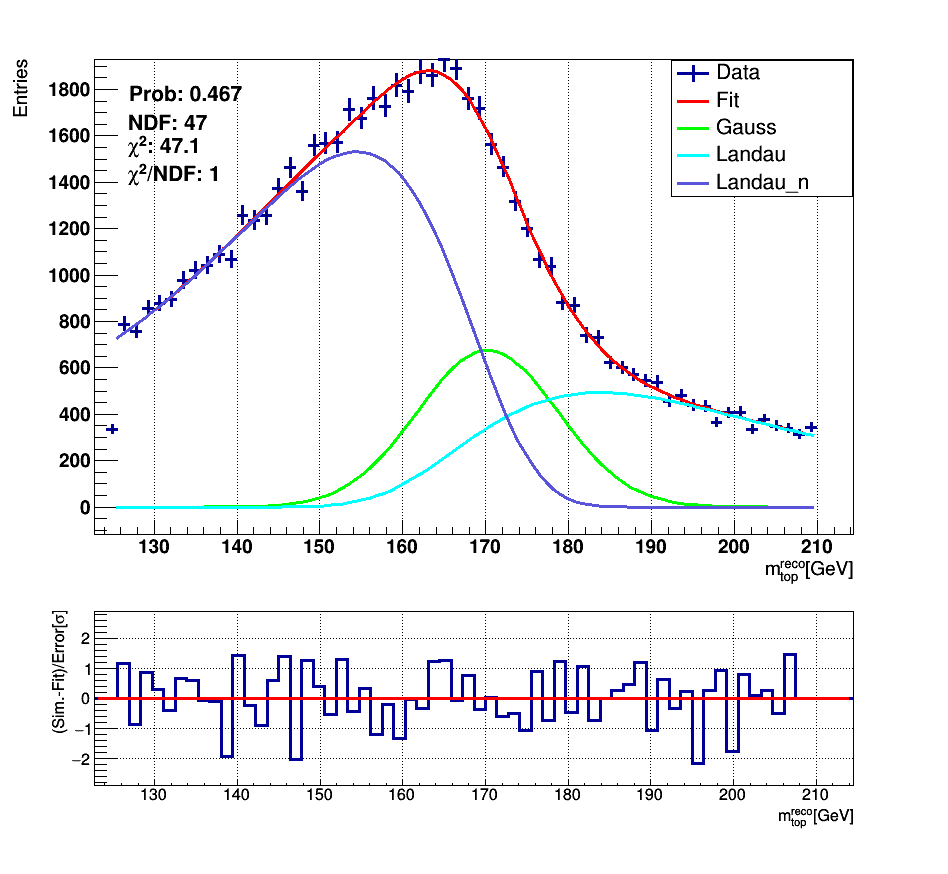
\includegraphics[width=0.725\linewidth]{PicsTop/170mtop.png}
		
		
	\end{textblock}	
	
	\begin{textblock}{7.5}(10.5,8.75)
		
		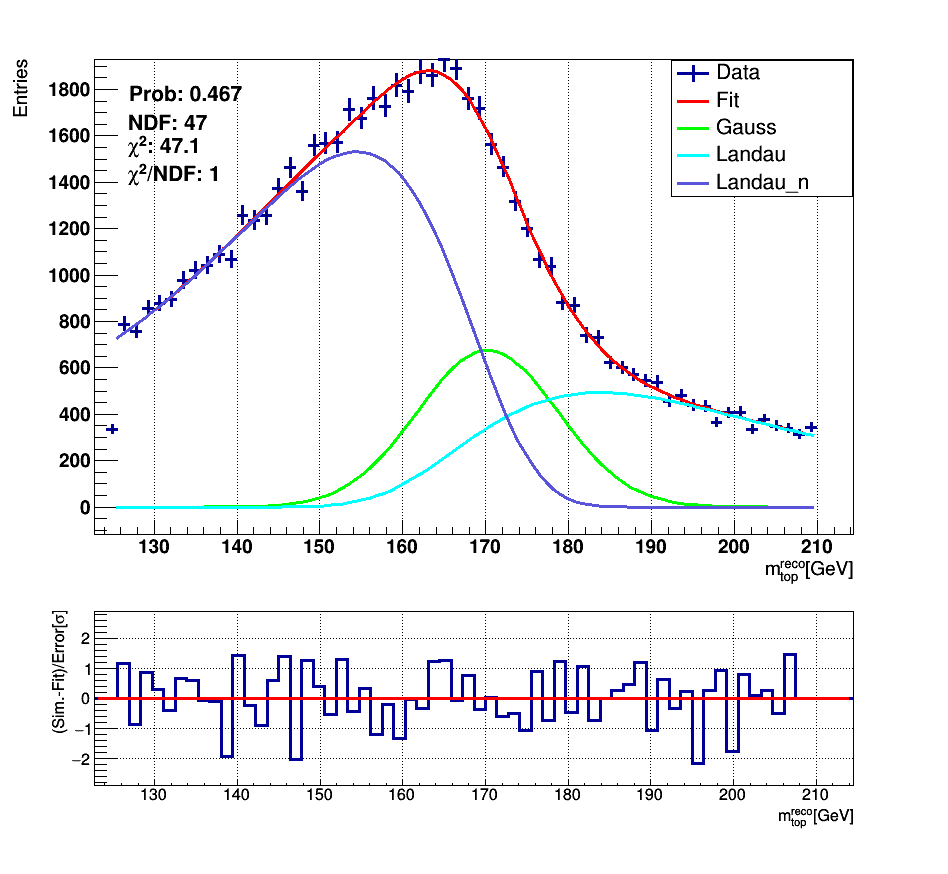
\includegraphics[width=0.725\linewidth]{PicsTop/170mtop.png}
		
		
	\end{textblock}	
	
	
	
	
}

\frame{
	\frametitle{\bfseries{Template fit functions}}
	\begin{textblock}{14.5}(2,3.25)
		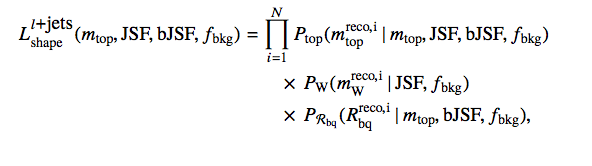
\includegraphics[width=0.725\linewidth]{PicsTop/Like}
	\end{textblock}
	\begin{textblock}{14.5}(2,7.25)
		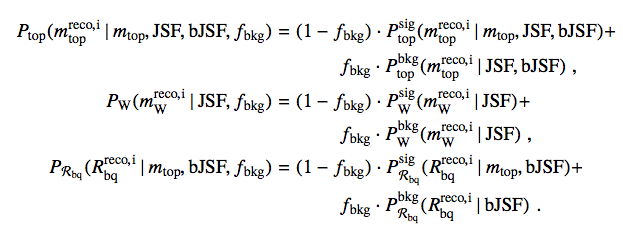
\includegraphics[width=0.725\linewidth]{PicsTop/Prob}
	\end{textblock}
	
}




\end{document}
